\documentclass[12pt]{article}
\usepackage[utf8]{inputenc}
\usepackage[english]{babel}

\usepackage{amsmath}
\usepackage{graphicx} 
\usepackage{caption}
\usepackage{subcaption}

\usepackage{geometry}
\geometry{left=2cm,  % margin for 2n pages
          right=2cm,  % margin for 2n+1 pages
          top=2cm,
          bottom=2cm}


\title{SPIM Excitation Lightpath Design with ABCD Matrix}
\author{\textbf{Borys Olifirov}\\Bogomoletz Institute of Physiology of NAS of Ukraine}
\date{}

\begin{document}
\maketitle


\section*{General light path design}

\begin{figure}[h]
    \centering
    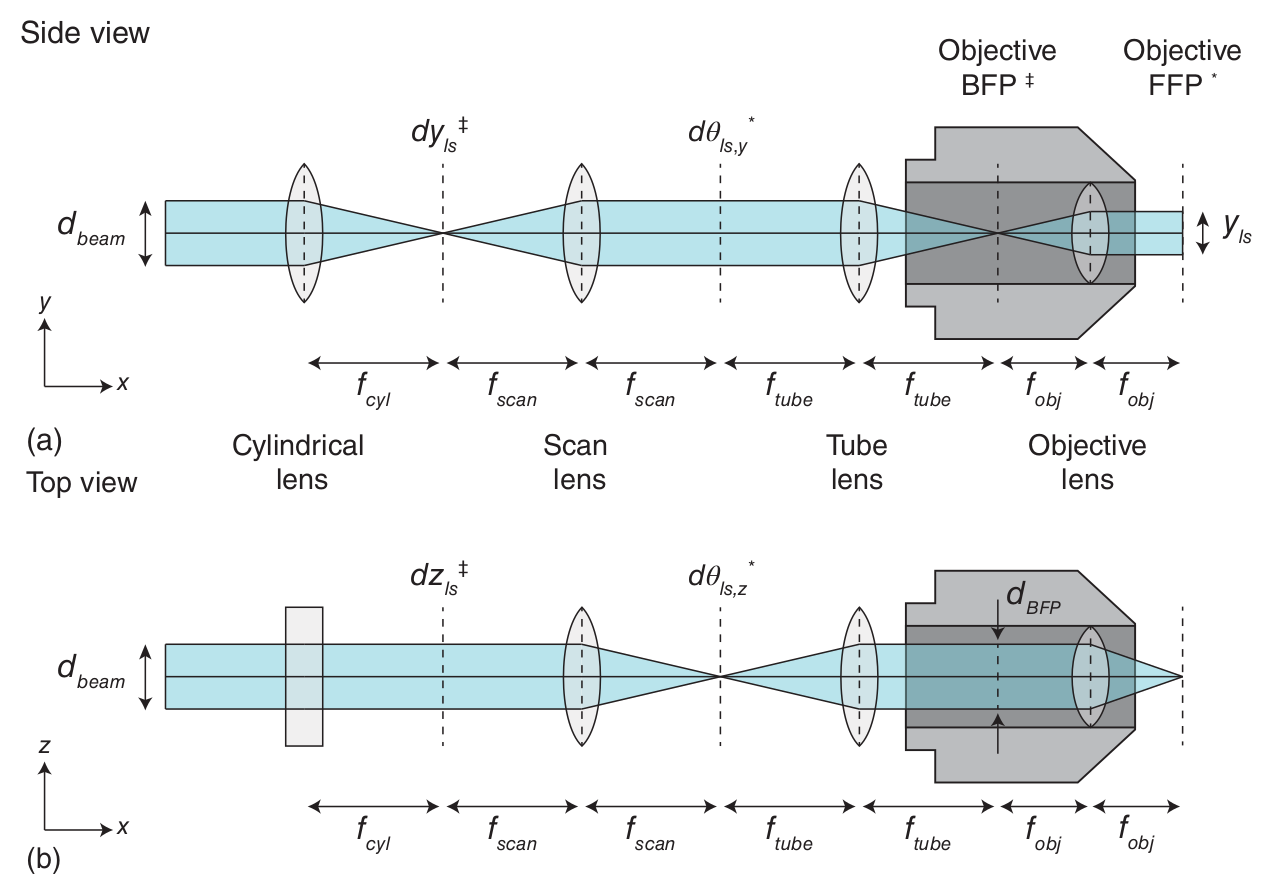
\includegraphics[width=0.9\textwidth]{../../4_pic/illumination_path.png}
    \caption{Relayed generation of a well-corrected static light sheet (\textit{Huisken et al., 2004})}
    \label{fig:your_label}
\end{figure}


\subsection*{Optical elements}

\begin{leftline}{}
  \begin{tabular}{ |c|c|c|c| }
    \hline
    Symbol & Parameters & Description & Part \# \\
    \hline
    $L_{cyl}$ & $f_{cyl} = 75 mm$ & Cylindrical lens & ThorLabs LJ1703RM-A \\
    $L_{scan}$ & $f_{scan} = 50 mm$ & Scaning lens & ThorLabs AC254-050-A \\
    $L_{tube}$ & $f_{tube} = 30 mm$ & Tube lens & ThorLabs AC254-030-A \\
    $L_{obj}$ & $f_{obj} = 45 mm$ & Objective 4X & Olympus PLT 4X, NA 0.1 \\
    \hline
  \end{tabular}
\end{leftline}


\subsection*{Element matrices}

\begin{equation}
\begin{split}
  M &= \begin{bmatrix} 1 & z_{obj} \\ 0 & 1 \end{bmatrix}
      \begin{bmatrix} 1 & 0 \\ -1/f_{obj} & 1 \end{bmatrix}
      \begin{bmatrix} 1 & f_{obj} + f_{tube} \\ 0 & 1 \end{bmatrix}
      \begin{bmatrix} 1 & 0 \\ -1/f_{tube} & 1 \end{bmatrix} \\
    &  \begin{bmatrix} 1 & f_{tube} + f_{scan} \\ 0 & 1 \end{bmatrix}
      \begin{bmatrix} 1 & 0 \\ -1/f_{scan} & 1 \end{bmatrix}
      \begin{bmatrix} 1 & f_{scan} + f_{cyl} \\ 0 & 1 \end{bmatrix}
      \begin{bmatrix} 1 & 0 \\ -1/f_{cyl} & 1 \end{bmatrix}
      \begin{bmatrix} 1 & z_{0} \\ 0 & 1 \end{bmatrix}
  \label{eq:gen_matrix}
\end{split}
\end{equation}


\begin{equation} 
    y_0 >= d_{beam} / 2
    \label{eq:max_y_0}
\end{equation}


\section*{Imaging chamber configuration}

\end{document}